%in_memory_file_system

\begin{figure}[t]
\begin{center}
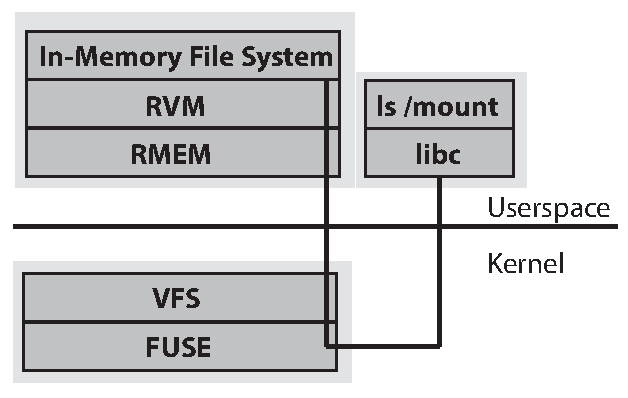
\includegraphics[scale=0.60]{inmem_fs_design.pdf}
\end{center}
\caption{In-memory file system design when using the RVM framework and FUSE library.}
\label{fig:inmem_fs_design}
\end{figure}

To demonstrate the flexibility and applicability of our framework we have
applied our framework to RvmFS, a VFS compliant in-memory file system (see
Figure~\ref{fig:inmem_fs_design}).  RvmFS uses main memory as the only storage
medium to provide very fast writes and reads.  To be able to use our framework
we have developed the file system using FUSE, a kernel module that allows the
creation of user-space file systems.  RvmFS performs a commit of the file
system in different situations: 1) an inode is created, 2) when a file is
closed and 3) when a {\emph sync} operation is performed.

To evaluate the performance of the system we ran a subset of the benchmarks in
the Filebench~\cite{filebench} benchmark suite.  We compare the performance of
the benchmark when running it against an ext4 file system backed by an SSD
drive and when running on RvmFS backed by a remote server.
Table~\ref{tab:description} describes each specific benchmark that we ran and
table~\ref{tab:results} shows the performance obtained.  We show the average
latency of each operation in each benchmark.

\begin{table}[h]
\centering
\caption{Description of the macro-benchmark tests used to evaluate RvmFS.}
\label{tab:description}
\resizebox{\columnwidth}{!}{%
    \begin{tabular}{ | l | c |} 
    \hline
    Benchmark name & Description \\
    \hline
    \hline
    \emph{file\_micro\_create}  & \pbox{20cm}{Create an empty file and issue 1024 appends of 1MB each} \\
    \hline
    \emph{ramdomread}  & \pbox{20cm}{Random reads (8K) from a file with size 1Mb} \\
    \hline
    \emph{openfiles}  &  \pbox{20cm}{Creates a fileset with 500 empty files, \\then proceeds to open each one.} \\
    \hline
    \end{tabular}
}
\end{table}

\begin{table}[t!]
\centering
\caption{Macro benchmark results of RvmFS}
\label{tab:results}
\resizebox{\columnwidth}{!}{%
  \begin{tabular}{ | l | c | c |} 
    \hline
    \pbox{20cm}{Benchmark\\ name} & \pbox{20cm}{Latency per Op. (SSD)} & \pbox{20cm}{Latency per Op. (RvmFS)} \\
    \hline
    \hline
    \emph{file\_micro\_create}  & append-file: 292us & 2967.7ms\\
    \hline
    \emph{randomread}  & Read: 25us & Read: 25us \\
    \hline
    \emph{openfiles}  & Open/close: 590us & Open: 2842us, Close: 740us \\
    \hline
  \end{tabular}
}
\end{table}

\paragraph{Discussion}

As shown in Table~\ref{tab:results}, RvmFS is considerably slower for some
specific benchmarks while obtaining similar performance in others.  The poor
performance of the file system stems from different reasons.  First, some of
the file system operations are not optimized for performance. For instance,
when extending a file length, RvmFS allocates a new region of memory and copies
all the file contents to the new region. Not only copying all the data is slow,
this also means that the next commit operation will backup the whole file
contents even if only a small part of the file changed.  Secondly, RvmFS
currently does not support multi-threaded access, common in modern file systems
such as ext4.  Thirdly, RvmFS is ultimately limited by the performance of RVM.
Due to the high overheads involved when backing up large contiguous regions of
memory in RVM, RvmFS suffers.  Finally, RvmFS is not built with locality of
storage in mind. This means that simple operations can touch many files.

Next we comment on the performance of each benchmark.

\paragraph{\bf \emph{file\_micro\_create}} The performance of RvmFS is far from
the performance of ext4. This has to do with the inefficiency of RvmFS when
extending the length of a file, as previously described.

\paragraph{\bf \emph{randomread}} In this benchmark RvmFS has similar
performance to the ext4 file system. Because the file being used to benchmark
the read operations is small it can fit in memory. This favours ext4, which can
rely on the kernel buffers to directly serve data.

\paragraph{\bf \emph{openfiles}} In this benchmark the close operation in RvmFS
is on par with the performance of ext4. On the other hand, the open operation
is roughly four times slower.

% filemicro_create.f ssd
% 1808: 2.081: Per-Operation Breakdown
% finish               512ops      512ops/s   0.0mb/s      0.0ms/op        0us/op-cpu [0ms - 0ms]
% append-file          513ops      513ops/s 511.9mb/s      0.3ms/op      292us/op-cpu [0ms - 0ms]
%  1808: 2.081: IO Summary:   513 ops, 512.938 ops/s, (0/513 r/w), 511.9mb/s,    351us cpu/op,   0.3ms latency

%filemicro_create.f with rvmfs
% 1890: 63.099: Per-Operation Breakdown
% finish               19ops        0ops/s   0.0mb/s      0.0ms/op        0us/op-cpu [0ms - 0ms]
% append-file          20ops        0ops/s   0.3mb/s   2967.7ms/op     8000us/op-cpu [0ms - 6087ms]
%  1890: 63.099: IO Summary:    20 ops, 0.333 ops/s, (0/0 r/w),   0.3mb/s, 3286000us cpu/op, 2967.7ms latency

% random read with rvmfs
%26236: 61.739: Per-Operation Breakdown
%rand-read1           2440621ops    40675ops/s 317.8mb/s      0.0ms/op       12us/op-cpu [0ms - 0ms]
%26236: 61.739: IO Summary: 2440621 ops, 40674.879 ops/s, (40675/0 r/w), 317.8mb/s,     25us cpu/op,   0.0ms latency

% Random read with ssd
%26602: 61.006: Per-Operation Breakdown
%rand-read1           2435691ops    40592ops/s 317.1mb/s      0.0ms/op       12us/op-cpu [0ms - 0ms]
%26602: 61.006: IO Summary: 2435691 ops, 40592.390 ops/s, (40592/0 r/w), 317.1mb/s,     25us cpu/op,   0.0ms latency

% openfiles with ssd
%28390: 62.200: Per-Operation Breakdown
%close1               1095781ops    18262ops/s   0.0mb/s      0.0ms/op      590us/op-cpu [0ms - 0ms]
%open1                1095788ops    18262ops/s   0.0mb/s      0.0ms/op      587us/op-cpu [0ms - 0ms]
%28390: 62.200: IO Summary: 2191569 ops, 36524.045 ops/s, (0/0 r/w),   0.0mb/s,      0us cpu/op,   0.0ms latency

% openfiles with rvmfs
%30196: 219.500: Per-Operation Breakdown
%close1               365ops        6ops/s   0.0mb/s   1196.5ms/op      740us/op-cpu [131ms - 6266ms]
%open1                366ops        6ops/s   0.0mb/s   1375.5ms/op     2842us/op-cpu [0ms - 6126ms]
%30196: 219.500: IO Summary:   731 ops, 12.183 ops/s, (0/0 r/w),   0.0mb/s,      0us cpu/op,   0.0ms latency
%30196: 219.500: Shutting down processes
%
